%!TEX root = ../dokumentation.tex

\chapter{Grundlagen}
In dem folgenden Kapitel werden die Grundlagen dieser Arbeit beschrieben. Zuerst wird das in dieser Arbeit verwendete \acs{VR}-Headset vorgestellt. Nach dem \acs{VR}-Headset folgt der Eye Tracker und zum Schluss die Laufzeit- und Entwicklungsumgebung Unity.

\section{Virtuelle Realität}
Die Grundidee der virtuellen Realität existiert bereits seit dem 19. Jahrhundert. David Brewester entwickelte 1848 ein linsenförmiges Stereoskop, welches das Gefühlt von Tiefe und Immersion hervorbrachte. Nennenswerte Entwicklungen im Bereich der virtuellen Realität wurden zu Beginn des 20. Jahrhunderts getätigt. \cite[S. 1f]{Singh.2017} 1987 gebrauchte der Informatiker Jaron Lanier als erster Wissenschaftler den Begriff \ac{VR} \cite{Doerner2019}. 

Bei der Suche einer einheitlichen Definition fällt eine große Diskrepanz in der Literatur auf. Die \citeauthor{BundeszentralefurpolitischeBildung.2018} definiert \ac{VR} als \glqq Darstellung und gleichzeitige Wahrnehmung der Wirklichkeit und ihrer physikalischen Eigenschaften in einer in Echtzeit computergenerierten, interaktiven virtuellen Umgebung\grqq  \cite{BundeszentralefurpolitischeBildung.2018}. \\
\citeauthor{LaValle.2019} von der University of Oulu definiert \ac{VR} als herbeiführen eines gezielten Verhaltens in einem Organismus durch künstliche sensorische Stimulation, während der Organismus sich der Störung kaum oder gar nicht bewusst ist \cite[S. 1]{LaValle.2019}. Aus seiner Definition kristallisiert \citeauthor{LaValle.2019} die folgenden vier Hauptkomponenten:\cite[S. 1,3]{LaValle.2019}
\begin{enumerate}
	\item \textbf{Gezieltes Verhalten}: Der Organismus hat eine Erfahrung (zum Beispiel Fliegen), welche durch den Entwickler erstellt wurde. 
	\item \textbf{Organismus}: Organismus bezieht sich hierbei auf den Benutzer von \ac{VR}, welcher jeglicher Lebensform entsprechen kann. Wissenschaftler setzten die \ac{VR}-Technologie bereits bei Fruchtfliegen, Kakerlaken, Fischen, Nagetiere und Affen ein. 
	\item \textbf{Künstliche sensorische Stimulation}: Der Einsatz moderner Technik ermöglicht das Replizieren verschiedener sensorischer Erlebnissen und das Ersetzen durch den Einsatz künstlicher Simulationen. 
	\item \textbf{Bewusstsein}: Bei einem \acl{VR} Erlebnis wird der Organismus entsprechend getäuscht, sodass sich dieser im Unterbewusstsein sowohl präsent als auch wohl in der virtuellen Welt fühlt.
\end{enumerate}

Die Mitgründer von der \citename{omnia.2017}{editor} \citename{omnia.2017}{author} definierten in ihrer Masterarbeit \ac{VR} als \glqq ein Medium, welches aus einer computergenerierten, interaktiven Welt besteht, die den Nutzer vollständig umgibt und durch die Ansprache ein oder mehrerer Sinne mittels geeigneter Systeme besonders immersiv erlebt werden kann\grqq \cite{omnia.2017}. Sie haben dabei nicht nur andere Definitionen betrachtet, sondern auch die Bedeutung der Wörter virtuell und Realität. Virtuell wird im Duden als \glqq nicht echt \grqq \cite{DudenVirtuell} oder als \glqq nicht in Wirklichkeit vorhanden, aber echt erscheinend\grqq \cite{DudenVirtuell} beschrieben. Ein Beispiel hierfür ist der virtuelle Speicher. Ein virtueller Speicher ist physisch nicht vorhanden, funktioniert aus Benutzersicht jedoch identisch wie ein physischer Speicher. Im Duden hat Realität unter anderem die Synonyme Wirklichkeit, Ernstfall und Leben \cite{DudenRealitaet}. Die Realität ist demzufolge \glqq die reale Welt, in die ein Mensch hineingeboren und die von ihm durch seine Sinneseindrücke wahrgenommen wird\grqq \cite{omnia.2017}.

Die \autoref{fig:mixed-reality} zeigt die Abgrenzung zwischen \ac{VR}, \ac{AR} und \ac{MR}. Während \ac{VR} einer virtuellen Umwelt dargestellt wird, wird bei \ac{AR} die reale Umwelt durch virtuelle Informationen erweitert. \ac{AR} sollte vielen nicht unbekannt sein, da \ac{AR} unter anderem beim Fußball bei einem Freistoß im TV-Bild angewendet wird. Im Bild wird eine Linie inklusive der Entfernung bis zum Tor dargestellt. \ac{MR} hingegen ist eine Technik, die sich sowohl aus \ac{AR} als auch aus \ac{VR} zusammensetzt. Sie vermischt eine reale Wahrnehmung mit einer künstlich erzeugten Wahrnehmung. \ac{MR} kann sowohl auf einer virtuellen Umgebung basieren, in die reale Informationen hinzugefügt werden, oder auf der realen Umgebung, in die virtuelle Objekte hinzugefügt werden, die fest in der Umgebung verankert werden und mit denen interagiert werden kann. \ac{MR} lässt sich mithilfe der von Microsoft entwickelten Datenbrille Hololens erleben. Mithilfe dieser Datenbrille wird die Umgebung um virtuelle Objekte erweitert, mit denen der Benutzer interagieren kann.
\begin{figure}[!htbp]
	\centering
	
\includegraphics[width=1\linewidth]{mixed-reality}
	\caption[Abgrenzung VR, AR und MR]{Abgrenzung VR, AR und MR \cite[S. 20]{BurofurTechnikfolgenAbschatzungbeimDeutschenBundestag.2019}}
	\label{fig:mixed-reality}
\end{figure}

\section{\acs{VR}-Headset}
Im Rahmen dieser Arbeit wird das \acs{VR}-Headset HTC Vive verwendet. Das Headset wurde gemeinsam von den Firmen HTC und Valve entwickelt. Das \acs{VR}-Headset lässt sich in die folgenden 3 Teile unterteilen. 

\subsection{\acl{HMD}}
\ac{HMD}

\begin{figure}[!htbp]
	\centering
	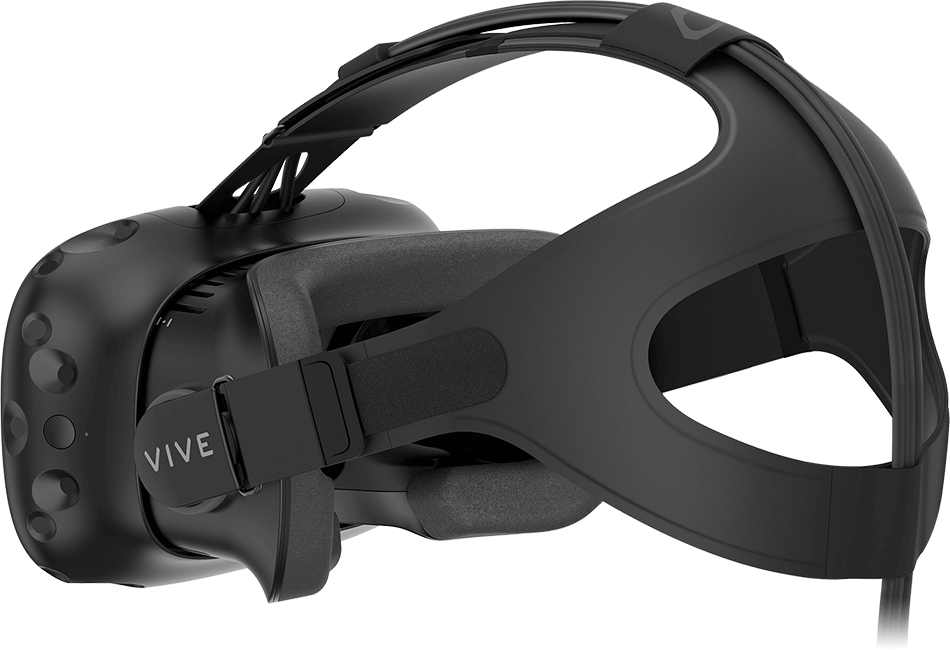
\includegraphics[width=0.5\linewidth]{vive-hardware-hmd-1}
	\caption[HTC Vive HMD]{HTC Vive \acs{HMD} \cite{ViveHMD}}
	\label{fig:vive-hardware-hmd-1}
\end{figure}

\todo{Abbildung von Headset}

\subsection{Controller}
\begin{figure}[!htbp]
	\centering
	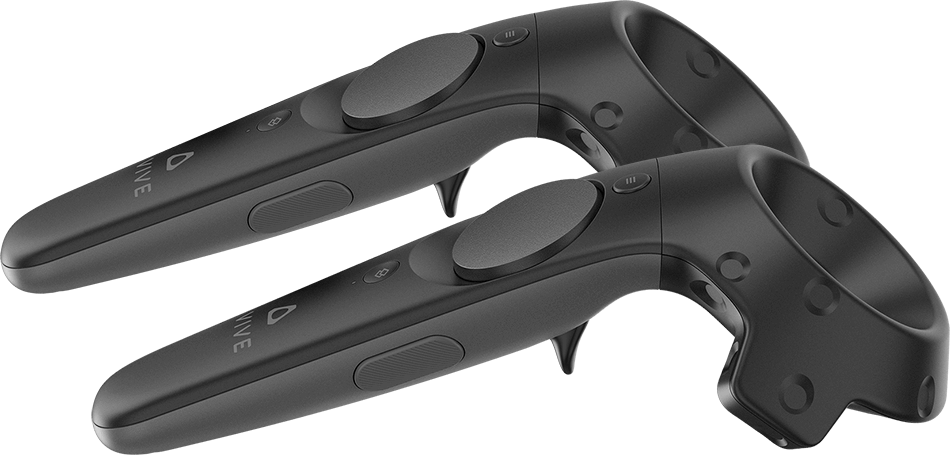
\includegraphics[width=0.5\linewidth]{vive-hardware-controllers-1}
	\caption[Controller der HTC Vive]{Controller der HTC Vive \cite{ViveControllers}}
	\label{fig:vive-hardware-controllers-1}
\end{figure}
\todo{Abbildung von Controller}

\subsection{Lighthouse Tracking System}
\begin{figure}[!htbp]
	\centering
	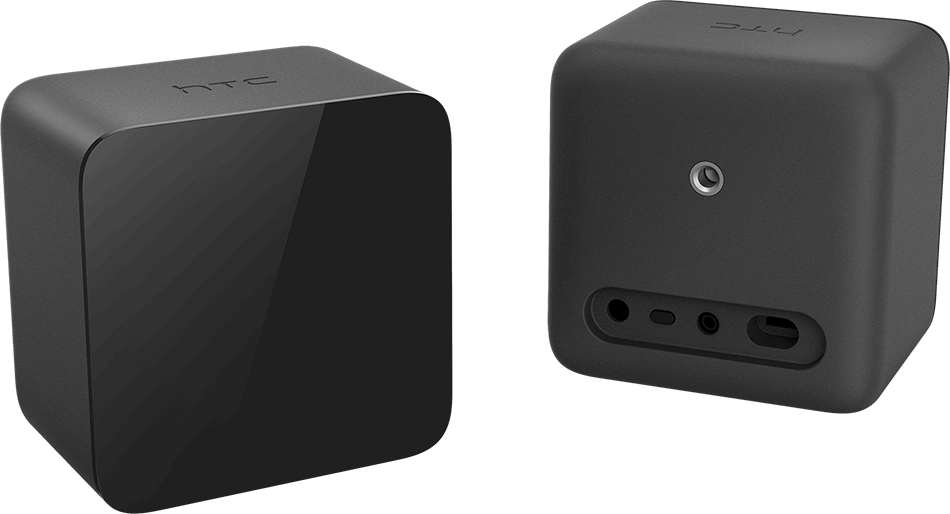
\includegraphics[width=0.5\linewidth]{vive-hardware-base-stations}
	\caption[Lighthouse Basis Station]{Lighthouse Basis Station \cite{ViveBaseStation}}
	\label{fig:vive-hardware-base-stations}
\end{figure}
\todo{Abbildung von Basisstation}

\begin{figure}[!htbp]
	\centering
	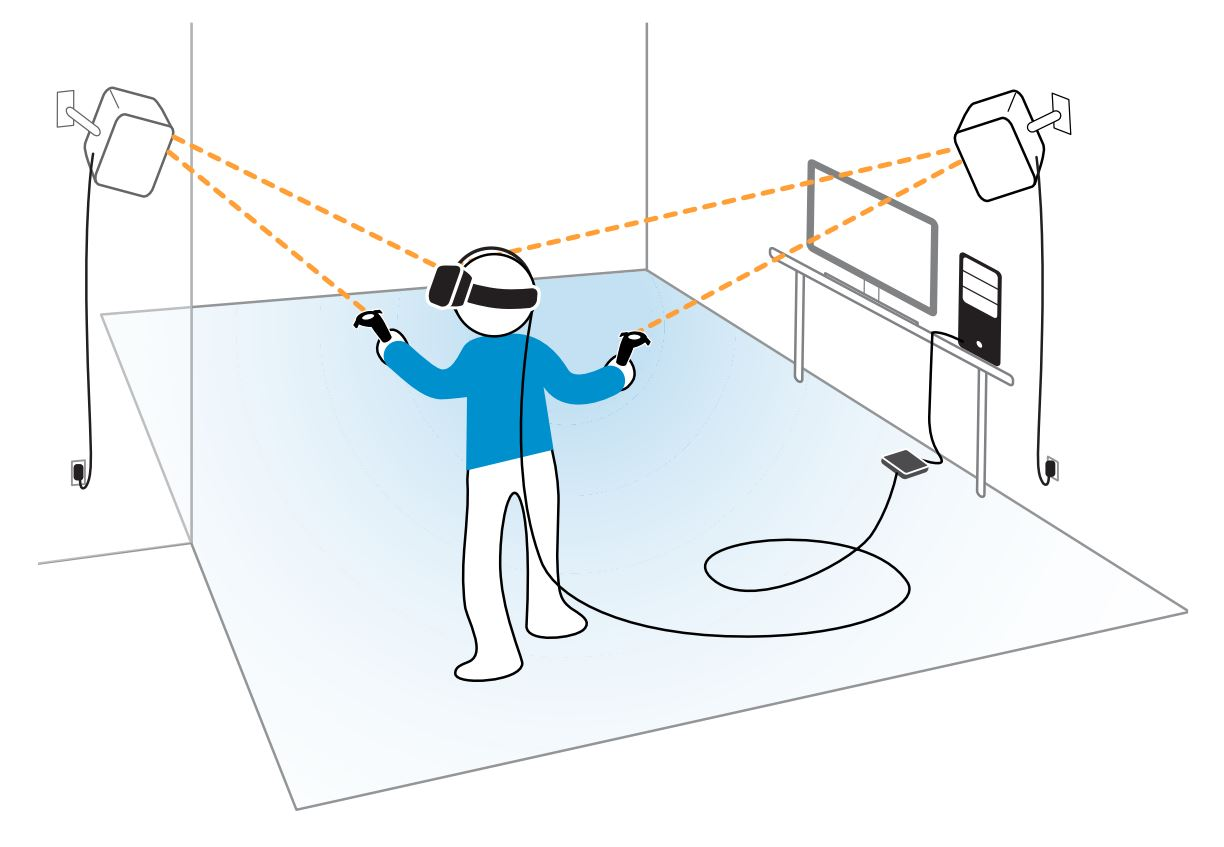
\includegraphics[width=1\linewidth]{graphic-tracking}
	\caption[Darstellung von VR mit dem Tracking von HMD und Controllern]{Darstellung von VR mit dem Tracking von HMD und Controllern \cite{VentureBeat}}
	\label{fig:graphic-tracking}
\end{figure}

\subsection{Systemvoraussetzungen}

\subsection{SteamVR}
\todo[inline]{Ein bissel was zu schreiben!}

\section{Eyetracking}
Eyetracking ist eine Technologie, die erkennt, in welche Richtung eine Person ihren Blick richtet. Hierfür werden beim Eyetracking Blick sowie Augenbewegungen erfasst. Die hauptsächlichen Parameter, die durch das Eyetracking erfasst werden, sind Fixiationen (von dem Benutzer fixierter Punkt oder Objekt), Sakkaden (schnelle Augenbewegungen bei der Erfassung eines neuen Fixpunktes) und Regression (Rücksprung zu vorherigen Fixpunkte oder Objekte).

\begin{figure}[!htbp]
	\centering
	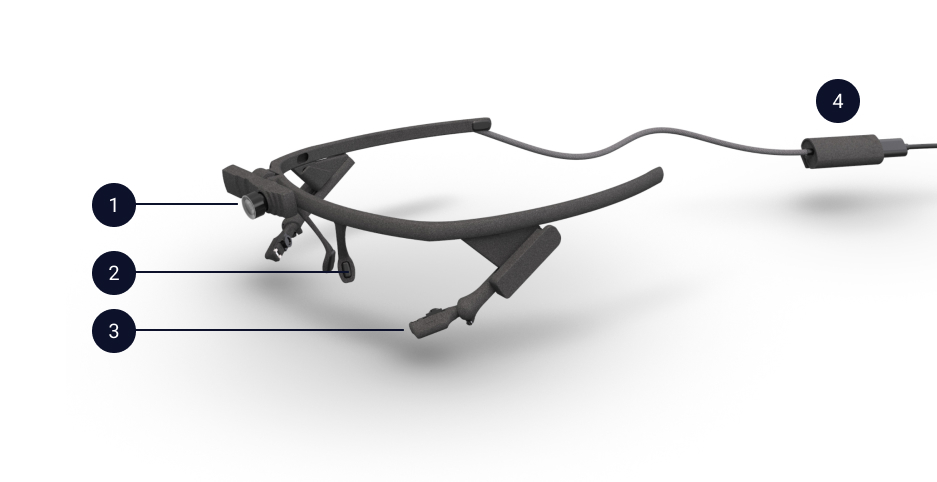
\includegraphics[width=0.75\linewidth]{pupil_labs_headset}
	\caption[Pupil Core Headset]{Pupil Core Headset \cite{PupilLabsHW}}
	\label{fig:pupil_labs_headset}
\end{figure}

Im Rahmen dieser Arbeit wird ein Eyetracker von Pupil Labs verwendet. Sie entwickeln seit 2014 die Plattform Pupil Core, die aus einer Open-Soure-Suite sowie dem Eyetracker besteht. In \autoref{fig:pupil_labs_headset} ist das tragbare Eyetracker Headset Pupil Core zu sehen, welches wie eine Brille getragen wird. An dem Headset ist eine Blickfeldkamera (Nummer 1) angebracht, welche das Blickfeld des Benutzers aufnimmt. \todo{Infrarot} Mithilfe der Augenkameras (Nummer 3) lässt sich das komplette Auge erfassen. Die Augenkameras lassen sich individuell auf die Augen einstellen. Ein USB-C Kabel (Nummer 4) dient als Stromversorgung sowie für den Austausch der Videodaten der Kameras. Wird der Eyetracker mit dem Computer verbunden, dann lässt sich mit der Pupil Core Software das Eyetracking starten. Mithilfe der Software lassen sich die Eyetracking-Daten aus den Videostreams auslesen, auswerten und über eine Netzwerk Schnittstelle zur Verfügung stellen. Zudem kann in das Umgebungsvideo der Blickfeldkamera der Punkt angezeigt werden, auf den der Benutzer seinen Blick fixiert. \\
Da in dieser Arbeit das Eyetracking innerhalb einer \ac{VR}-Umgebung untersucht werden soll, wird ein speziell für die HTC Vive entwickelter Eyetracker von Pupil Labs verwendet. Dies ist ein Add-on von Pupil Labs, welches in das HTC Vive Headset eingebaut wird und während dem Tragen des Headsets verwendet werden kann. In \autoref{fig:pupil_labs_addon} ist das Add-on von Pupil Labs und das \ac{VR}-Headset HTC Vive dargestellt. Das Add-on wird in die Innenseite um die Linsen des Headsets angebracht. 

\begin{figure}[!htbp]
	\centering
	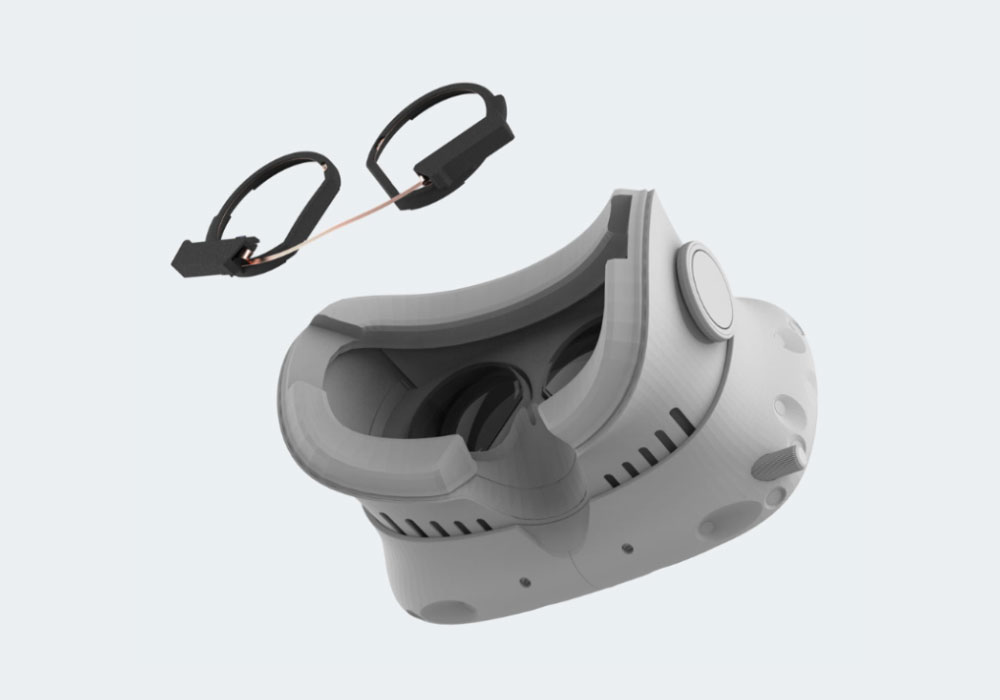
\includegraphics[width=0.5\linewidth]{vive-addon}
	\caption[Pupil Core Add-on für HTC Vive]{Pupil Core Add-on für HTC Vive \cite{PupilLabsAddOn}}
	\label{fig:pupil_labs_addon}
\end{figure}

\todo{Zugriff auf Daten}
\cite{Clay_Koenig_Koenig_2019}

\cite{Kassner_2014}

\section{Unity}
Standardmäßig entspricht 1 Einheit 1 Meter (siehe \cite{BrentAllard.2017} \& \cite{AVividLight.2010}) --> Aussage ist plausibel, da standardmäßig in den Projekteinstellungen bei Physics die Gravitation auf -9,81 gesetzt ist.

\subsection{steamVR}

\subsection{hmd\_eyes}

\section{Fitts' Law}